\documentclass[10pt]{article}

%\usepackage{revnum}

\usepackage{fancyhdr}
\usepackage{amsmath,amssymb,amsfonts}
\usepackage{graphicx}
\usepackage[utf8]{inputenc}
\usepackage{hyperref}
\usepackage{subfig}
\usepackage{fontawesome}

\oddsidemargin  0.25in
\evensidemargin 0.25in
\textwidth      6.3in
\topmargin      -0.25in
\textheight     8.7in
\parskip        0.1in
\parindent      0.0in

\hyphenation{}

\begin{document}
\begin{center}
{\huge Juan Irving Vásquez Gómez}
\vspace{0.5cm}


\begin{minipage}[b]{0.30\linewidth}
	\centering
%	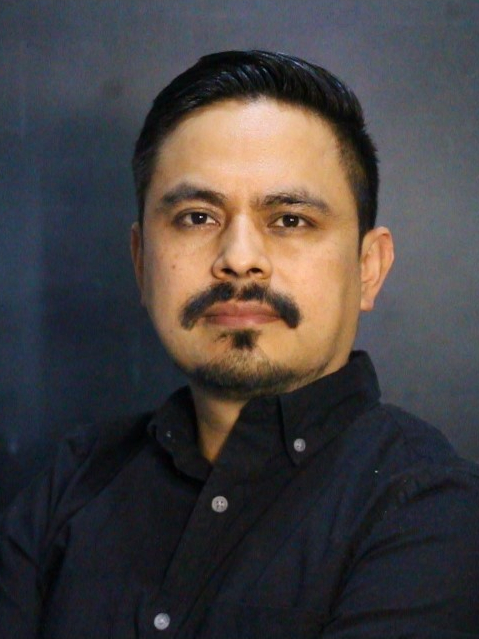
\includegraphics[width=\textwidth]{jivg36}
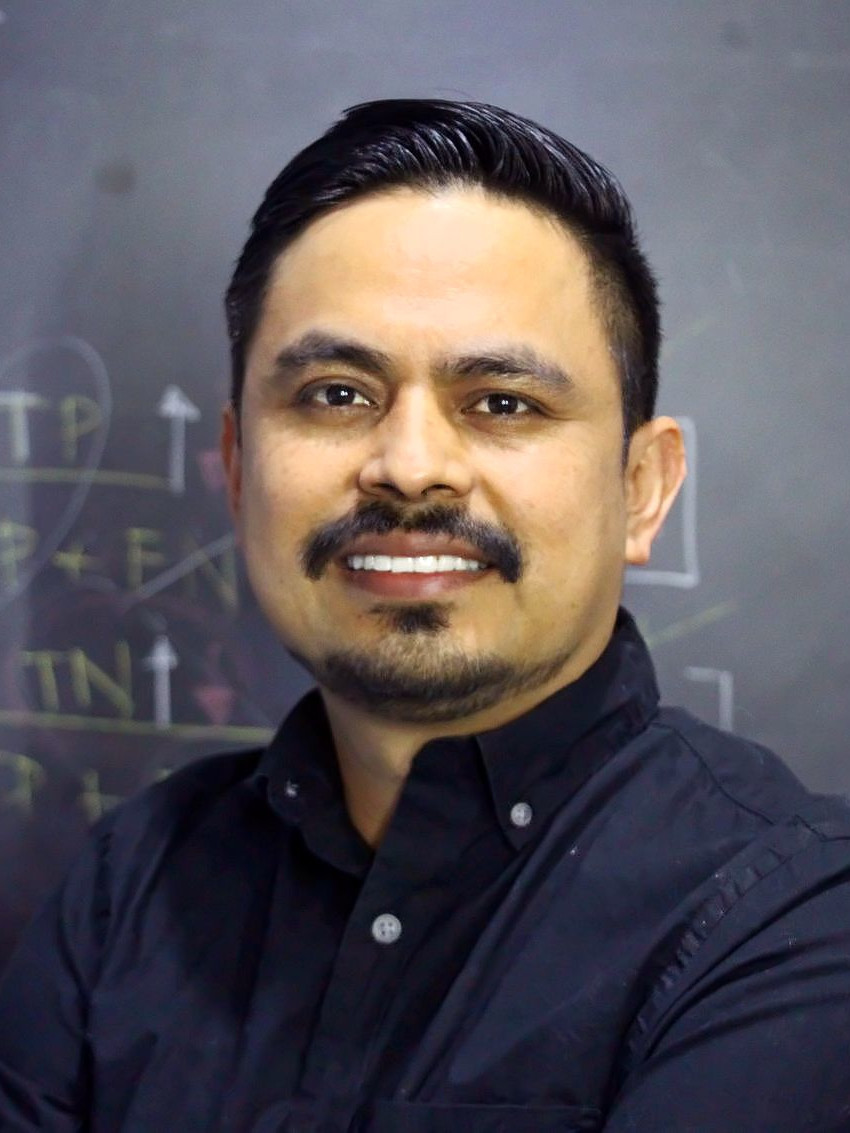
\includegraphics[width=\textwidth]{jivg_foto2}
%	\caption{default}
%	\label{fig:figure1}
\end{minipage}
\hspace{0.5cm}
\begin{minipage}[b]{0.65\linewidth}
\textbf{Fecha de Nacimiento:} Noviembre, 1984 \\
\textbf{Trabajo:} Profesor Investigador Titular C. Instituto Politécnico Nacional (IPN), Centro de Innovación y Desarrollo Tecnológico en Cómputo (CIDETEC) \href{https://www.cidetec.ipn.mx/}{\faExternalLink} \\ 
\textbf{Dirección:} Av."Juan de Dios Bátiz" s/n esq. Miguel Othón de Mendizábal, 
Col. Nueva Industrial Vallejo, Del. Gustavo A. Madero, Ciudad de México, C.P. 07700. \\
\textbf{Teléfono \faPhone:} +52 55 5729-6000 Ext. 52516. \\
\textbf{email \faEnvelopeO:} jvasquezg[en]ipn.mx, jirvingvg[en]gmail.com\\
\textbf{URL \faExternalLink:} \url{https://jivg.org} \\
\textbf{ORCID:} \url{https://orcid.org/0000-0001-8427-9333}\\
\textbf{Scopus Id:} \href{https://www.scopus.com/authid/detail.uri?authorId=54415023500}{54415023500}\\
\textbf{github \faGithub :} \url{https://github.com/irvingvasquez} \\
\textbf{Kaggle:} \url{https://www.kaggle.com/irvingvasquez}\\
\end{minipage}

\end{center}

\begin{center}
{\bf Intereses de investigación:} \\ Aprendizaje profundo, visión computacional, robótica, planificación de movimientos, reconstrucción tridimensional y conservación de áreas naturales protegidas. 
\end{center}

{\bf SÍNTESIS PERSONAL}
\vspace{3pt}
\hrule

``Soy un investigador científico apasionado por comprender los algoritmos que involucran la interacción de la visión computacional con la robótica. Mi formación como científico e ingeniero en computación me ha permitido investigar analíticamente los algoritmos involucrados así como llevarlos a la solución de problemas prácticos. Mis intereses actuales de investigación son la visión basada en aprendizaje profundo, la planificación de trayectorias en robots móviles y la exploración/reconstrucción autónoma de ambientes u objetos."
 \\

{\bf CONTRIBUCION CIENTÍFICA} 
\vspace{3pt}
\hrule

Mi investigación ha contribuido a entender la relación existente entre un modelo geométrico y la pose de un sensor que tiene que observarlo. En el caso de un modelo geométrico bi-dimensional conocido he demostrado analíticamente que un algoritmo basado en los calipers rotativos obtiene un camino óptimo de observación con complejidad lineal. En el caso un modelo tri-dimensional desconocido fui uno de los primeros investigadores en mostrar evidencia que es factible estimar las poses del sensor que lo observa usando un enfoque basado en datos. \\

{\bf BIOGRAFÍA RESUMIDA}
\vspace{3pt}
\hrule

J. Irving Vasquez recibió los grados de maestría en ciencias y doctorado en ciencias por el Instituto Nacional de Astrofísica Óptica y Electrónica (INAOE) en 2009 y 2014 respectivamente. El grado de Ingeniero en Sistemas Computacionales lo adquirió por el Instituto Tecnológico de Tehuacán en 2006. Desde febrero de 2016 se desepeña como catedrático CONACYT asignado al Instituto Politécnico Nacional. Su producción científica incluye diversas publicaciones en revistas arbitradas y congresos internacionales, así como desarrollos tecnológicos aplicados a la industria. Sus intereses actuales de investigación incluyen visión computacional, robótica, planificación de movimientos, mapeo y sus aplicaciones a vehículos autónomos, reconstrucción tridimensional de objectos, inspección entre otras. \\
	
{\bf EDUCACIÓN}
\vspace{3pt}
\hrule

\begin{minipage}{1.5 in}
	2014\\
\end{minipage}
\begin{minipage}{4.5in}
	\textbf{Doctorado en ciencias computacionales.} \textit{Instituto Nacional de Astrofísica Óptica y Electrónica (INAOE) \href{https://www.inaoep.mx/}{\faExternalLink}.} Tesis: Planificación de vistas para reconstrucción tridimensional de objectos con robots móviles \href{https://jivasquez.files.wordpress.com/2015/03/tesis-doctorado.pdf}{\faFilePdfO}. Directores: Enrique Sucar y Rafael Murrieta.\\ 
\end{minipage}

\begin{minipage}{1.5 in}
	2009\\
\end{minipage}
\begin{minipage}{4.5in}
	\textbf{Maestría en ciencias computacionales.} \textit{Instituto Nacional de Astrofísica Óptica y Electrónica (INAOE) \href{https://www.inaoep.mx/}{\faExternalLink}.} Tesis: Planificación de vistas para reconstrucción tridimensional de objetos \href{https://jivasquez.files.wordpress.com/2015/03/tesis-maestria.pdf}{\faFilePdfO}. Directores: Enrique Sucar y Efraín López-Damián.\\ 
\end{minipage}

\begin{minipage}{1.5 in}
	2006\\
\end{minipage}
\begin{minipage}{4.5in}
	\textbf{Ingeniería en sistemas computacionales} \textit{Instituto Tecnológico de Tehuacán (ITT)} \href{http://www.ittehuacan.edu.mx/}{\faExternalLink}. Graduado por ``Promedio de excelencia".\\ 
\end{minipage} 


{\bf EXPERIENCIA PROFESIONAL}
\vspace{3pt}
\hrule

\begin{minipage}{1.5 in}
	10/2021 - Actual\\
\end{minipage}
\begin{minipage}{4.5in}
	\textbf{Profesor titular.} Centro de Innovación y Desarrollo Tecnológico en Cómputo. Instituto Politécnico Nacional (IPN).\\ 
\end{minipage}

\begin{minipage}{1.5 in}
	02/2016 - 09/2021\\
\end{minipage}
\begin{minipage}{4.5in}
	\textbf{Cátedra CONACyT} asignado al Instituto Politécnico Nacional (IPN), Centro de Innovación y Desarrollo Tecnológico en Cómputo (CIDETEC). Proyecto 1507.\\ 
\end{minipage}

%\begin{minipage}{1.5 in}
%	01/2015 - 12/2015\\
%\end{minipage}
%\begin{minipage}{4.5in}
%	CONACYT Research Fellow assigned to Instituto Politécnico Nacional, Centro de Innovación y Desarrollo Tecnológico en Cómputo. Project 1507.\\ 
%\end{minipage}

\begin{minipage}{1.5 in}
	01/2015 - 11/2015\\
\end{minipage}
\begin{minipage}{4.5in}
	\textbf{Investigador posdoctoral} en el proyecto ``Agricultura de precisión por análisis multiespectral
	utilizando vehículos aéreos no tripulados". Instituto Nacional de Astrofísica Óptica y Electrónica. Proyecto CONACYT 222035, Responsable técnico: Enrique Muñoz de Cote\\ 
\end{minipage}

\begin{minipage}{1.5 in}
08/2009 - 08/2014\\
\end{minipage}
\begin{minipage}{4.5in}
\textbf{Programador} del equipo Markovito-INAOE en la competición Robocup@home del Torneo Mexicano de Robótica.\\ 
\end{minipage}

{\bf PREMIOS Y DISTINCIONES}
\vspace{3pt}
\hrule


\begin{minipage}{1.5 in}
	2017 - 2019\\
\end{minipage}
\begin{minipage}{4.5in}
	Candidato a Investigador Nacional otorgado por el Consejo Nacional de Ciencia y Tecnología, México\\ 
\end{minipage}

\begin{minipage}{1.5 in}
	2020 - 2022\\
\end{minipage}
\begin{minipage}{4.5in}
	Investigador Nacional Nivel 1 otorgado por el Consejo Nacional de Ciencia y Tecnología, México\\ 
\end{minipage} 

{\bf PUBLICACIONES}
\vspace{3pt}
\hrule

\begin{figure}[t]
	\subfloat[Distribuci\'on de productos.\label{subfig-1:dummy}]{%
		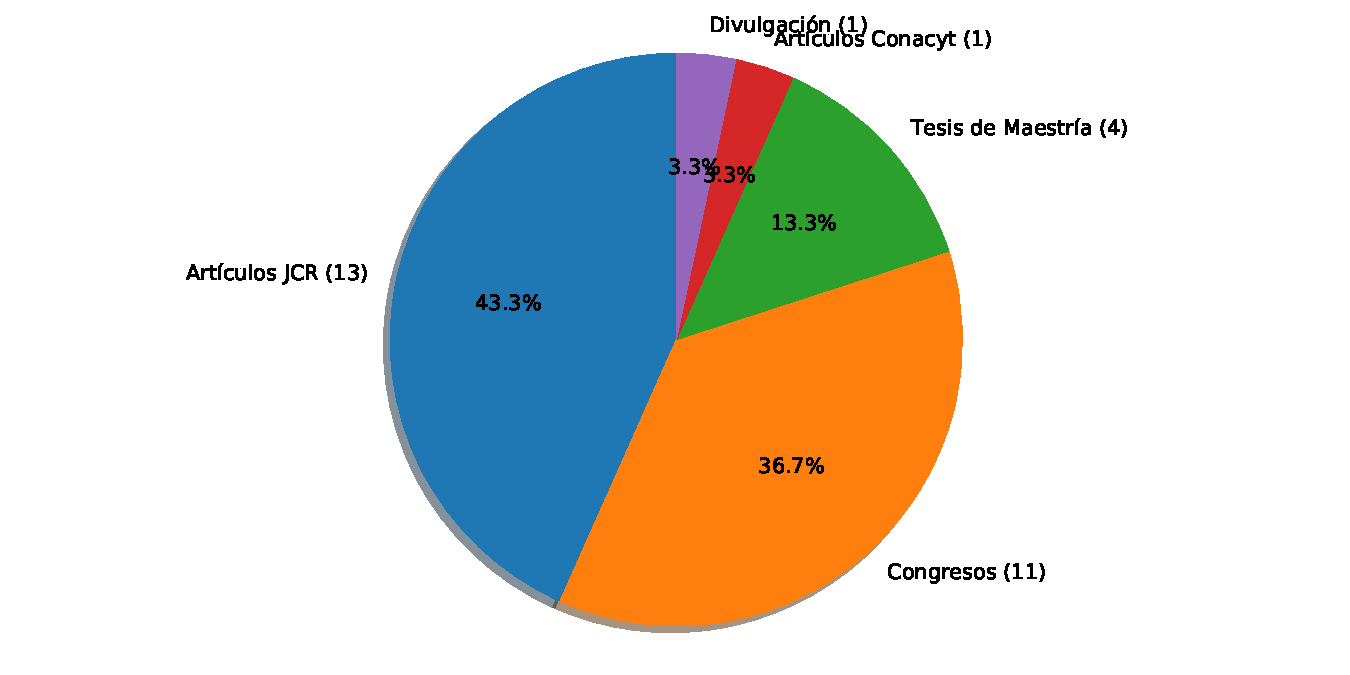
\includegraphics[trim=70 0 70 0, clip, width=0.60\textwidth]{../text/products.pdf}
	}
		\subfloat[Métricas en Scopus \href{https://www.scopus.com/authid/detail.uri?authorId=54415023500}{\faExternalLink} \label{subfig-2:dummy}]{%
			\begin{tabular}{|ll}
				Documentos: & 31  \\
				Citas:      & 574 \\
				Índice H:   & 13 
			\end{tabular}
	}
	\caption{Gráficas sobre la producción científica.}
	\label{fig:dummy}
\end{figure}

%\begin{figure}[h]
%	\centering
%	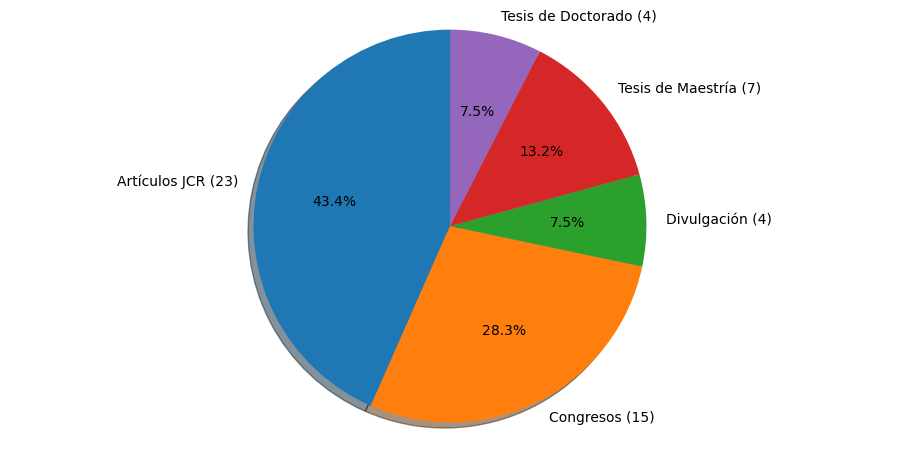
\includegraphics[width=0.7\linewidth]{../text/products}
%	\caption{Distribución de publicaciones.}
%	\label{fig:products}
%\end{figure}

\begin{itemize}
	\item \textbf{Artículos en revistas indexadas en el JCR:}
	\begin{itemize} 
\item L{\'o}pez-Jim{\'e}nez, Efren and Vasquez-Gomez, Juan Irving and Sanchez-Acevedo, Miguel Angel and Herrera-Lozada, Juan Carlos and Uriarte-Arcia, Abril Valeria, Columnar cactus recognition in aerial images using a deep learning approach,\textit{ Ecological Informatics,} (2019), I.F. 2.310 
\item Vasquez-Gomez, Juan Irving and Marciano-Melchor, Magdalena and Valentin, Luis and Herrera-Lozada, Juan Carlos, Coverage Path Planning for 2D Convex Regions,\textit{ Journal of Intelligent and Robotic Systems,} (2019), I.F. 2.020 
\item Vasquez-Gomez, J Irving and Sucar, L Enrique and Murrieta-Cid, Rafael and Herrera-Lozada, Juan-Carlos, Tree-based search of the next best view/state for three-dimensional object reconstruction,\textit{ International Journal of Advanced Robotic Systems,} (2018), I.F. 1.223 
\item Yervilla-Herrera, Heikel and Vasquez-Gomez, J Irving and Murrieta-Cid, Rafael and Becerra, Israel and Sucar, L Enrique, Optimal motion planning and stopping test for 3-D object reconstruction,\textit{ Intelligent Service Robotics,} (2018), I.F. 1.346 
\item Vasquez-Gomez, J Irving and Sucar, L Enrique and Murrieta-Cid, Rafael, View/state planning for three-dimensional object reconstruction under uncertainty,\textit{ Autonomous Robots,} (2017), I.F. 2.244 
\item Vasquez-Gomez, J Irving and Sucar, L Enrique and Murrieta-Cid, Rafael and Lopez-Damian, Efrain, Volumetric next-best-view planning for 3d object reconstruction with positioning error,\textit{ International Journal of Advanced Robotic Systems,} (2014), I.F. 0.526 
\end{itemize} 

	
	\item \textbf{Artículos en revistas indexadas en el índice CONACyT:}
	\begin{itemize} 
\item Olguin Carbajal, Mauricio and Herrera-Lozada, Juan Carlos and Rivera-Z{\'a}rate, Israel and Serrano-Talamantes, J Felix and Cadena-Mart{\'\i}nez, Rodrigo and V{\'a}squez-G{\'o}mez, J Irving, Minimum Addition Chains Generation Using Evolutionary Strategies,\textit{ Computaci{\'o}n y Sistemas,} (2018) 
\end{itemize} 

	
	\item \textbf{Artículos en conferencias internacionales:}
	\begin{itemize} 
\item Rodr{\'\i}guez-Hernandez, Erick and Vasquez-Gomez, Juan Irving and Herrera-Lozada, Juan Carlos, Flying through Gates using a Behavioral Cloning Approach, \textit{ 2019 International Conference on Unmanned Aircraft Systems (ICUAS),} 2019 
\item Vasquez-Gomez, Juan Irving and Herrera-Lozada, Juan-Carlos and Olguin-Carbajal, Mauricio, Coverage path planning for surveying disjoint areas, \textit{ 2018 International Conference on Unmanned Aircraft Systems (ICUAS),} 2018 
\item Vasquez-Gomez, Juan Irving and Herrera-Lozada, Juan Carlos and Olguin-Carbajal, Mauricio, Spatial resolution optimization for terrain coverage with UAVs, \textit{ 2017 International Conference on Mechatronics, Electronics and Automotive Engineering (ICMEAE),} 2017 
\item Vasquez-Gomez, Juan Irving and Melchor, Magdalena Marciano and Lozada, Juan Carlos Herrera, Optimal coverage path planning based on the rotating calipers algorithm, \textit{ 2017 International Conference on Mechatronics, Electronics and Automotive Engineering (ICMEAE),} 2017 
\item Vasquez-Gomez, J Irving and Gomez-Casta{\~n}eda, Cecilia and De Cote, Enrique Mu{\~n}oz and Herrera-Lozada, Juan Carlos, Multirotor uav coverage planning under wind conditions, \textit{ 2016 International Conference on Mechatronics, Electronics and Automotive Engineering (ICMEAE),} 2016 
\item Vasquez-Gomez, J Irving and Sucar, L Enrique and Murrieta-Cid, Rafael, View planning for 3d object reconstruction with a mobile manipulator robot, \textit{ 2014 IEEE/RSJ International Conference on Intelligent Robots and Systems (IROS),} 2014 
\item Vasquez-Gomez, J Irving and Sucar, L Enrique and Murrieta-Cid, Rafael, Hierarchical ray tracing for fast volumetric next-best-view planning, \textit{ 2013 International Conference on Computer and Robot Vision (CRV),} 2013 
\item V{\'a}squez, Juan Irving and Sucar, L Enrique, Next-best-view planning for 3d object reconstruction under positioning error, \textit{ Mexican International Conference on Artificial Intelligence (MICAI),} 2011 
\item V{\'a}squez-G{\'o}mez, Juan Irving and L{\"o}pez-Damian, Efra{\'\i}n and Sucar, Luis Enrique, View planning for 3D object reconstruction, \textit{ 2009 IEEE/RSJ International Conference on Intelligent Robots and Systems (IROS),} 2009 
\end{itemize} 

	
	\item \textbf{Preprints:}
	\begin{itemize} 
\item Vazquez-Carmona, E. Viridiana and Vasquez-Gomez, J. Irving and Herrera Lozada, Juan Carlos and Antonio-Cruz, Mayra, Coverage Path Planning for Spraying Drones, Under review in CAIE, 2021, \href{https://arxiv.org/abs/2105.08743}{\faFilePdfO} 
\item Uriarte-Arcia, Abril; Vasquez, Juan; Taud, Hind; Garcia-Floriano, Andrés; Ventura-Molina, Elias, Coast Sargassum Level Estimation from Smartphone Pictures, Submitted to Methods in Ecology and Evolution, 2021, \href{https://arxiv.org/abs/3939932}{\faFilePdfO} 
\end{itemize} 

\end{itemize} 

\vspace{0.3cm}
\textbf{PROYECTOS Y DESARROLLOS TECNOLÓGICOS}
\vspace{3pt}
\hrule
\begin{itemize}
	\item \textbf{Proyectos.}
	\begin{itemize}
\item 2021-2022 \textit{Asistencia al monitoreo ambiental}, Proyectos de investigación en Inteligencia Artificial en el Espacio de Innovación UNAM – HUAWEI.
\end{itemize}

	\item \textbf{Desarrollos validados por la comisión transversal de tecnología del SNI.}
	\begin{itemize} 
\item 2016, \textit{ Planificación de Vuelo de Vehiculos Aéreos no Tripulados para Agricultura de Precisión. Proyecto CONACYT 222035,} Verstand Technologies, Hermosillo Sonora, México, Reserved License, Validada por la comisión transversal de tecnología del SNI en 2019. 
\end{itemize} 

\end{itemize}


\vspace{0.3cm}
{\bf FORMACIÓN DE RECURSOS HUMANOS}
\vspace{3pt}
\hrule

\begin{itemize}
	\item Estudiantes graduados de maestría:
	\begin{itemize} 
\item Rodriguez Hernandez, Erick, \textit{ Clonaci\'on de comportamiento para cruce de pasajes estrechos con VANT,} 2019 
\item Jim{\'e}nez, Efr{\'e}n L{\'o}pez, \textit{ Sistema embebido para la supervisi{\'o}n inteligente de terrenos con veh{\i}culos a{\'e}reos no tripulados,} 2018 
\item Mendoza Guadarrama, Miguel, \textit{ NBV-Net: Una red neuronal para calcular la siguiente mejor vista,} 2018 
\end{itemize} 


	\item Estudiantes graduados de doctorado:
	\begin{itemize} 
\item Esther-Viridiana Vazquez Carmona, \textit{ Diseño de un algoritmo de cobertura de espacios tridimensionales para vehículos aéreos no tripulados }, \href{ https://jivg.org/wp-content/uploads/2023/02/2023_phd_Vazquez.pdf }{\faFilePdfO}, 2023, Instituto Politécnico Nacional. 
\item Erick Rodríguez Hernández, \textit{ Navegación autónoma para vehículos en pistas cerradas con obstáculos móviles }, \href{ https://jivg.org/wp-content/uploads/2022/08/2022_phd_Rodriguez.pdf }{\faFilePdfO}, 2022, Instituto Politécnico Nacional. 
\end{itemize} 

	
	\item Clases impartidas (últimos años):
	\begin{itemize} 
\item 2017/01/01, \textit{ Seminario Departamental I,} nivel Maestría, 36 horas. 
\item 2017/01/01, \textit{ Seminario Departamental II,} nivel Maestría, 36 horas. 
\item 2017/01/01, \textit{ Temas Selectos en Tecnología de Cómputo,} nivel Maestría, 72 horas. 
\item 2017/01/01, \textit{ Visión Artificial,} nivel Maestría, 72 horas. 
\item 2017/08/01, \textit{ Visión 3D,} nivel Maestría, 72 horas. 
\item 2017/08/01, \textit{ Seminario Departamental II,} nivel Maestría, 36 horas. 
\item 2017/08/01, \textit{ Seminario Departamental III,} nivel Maestría, 36 horas. 
\item 2018/01/01, \textit{ Seminario Departamental II,} nivel Maestría, 36 horas. 
\item 2018/01/01, \textit{ Seminario Departamental III,} nivel Maestría, 36 horas. 
\item 2018/01/01, \textit{ Temas Selectos en Tecnología de Cómputo,} nivel Maestría, 72 horas. 
\item 2018/08/01, \textit{ Seminario Departamental III,} nivel Maestría, 36 horas. 
\item 2018/08/01, \textit{ Visión Artificial,} nivel Maestría, 72 horas. 
\item 2018/08/01, \textit{ Temas Selectos en Tecnología de Cómputo,} nivel Maestría, 72 horas. 
\item 2019/01/01, \textit{ Visión Artificial,} nivel Maestría, 72 horas. 
\item 2019/01/01, \textit{ Temas Selectos en Tecnología de Cómputo,} nivel Maestría, 72 horas. 
\end{itemize} 

\end{itemize}


\vspace{0.3cm}
\textbf{VINCULACIÓN Y DIVULGACIÓN}
\vspace{3pt}
\hrule

\begin{itemize}
	\item Pláticas impartidas:
	\begin{itemize} 
\item 2019/10/02, The view planning problem from the mahine learning perspective, en \textit{ Taller conjunto sobre Deep Learning y Ciencia de Datos CIMAT-INAOE,} Centro de Investigación en Matemáticas (CIMAT), Guanajuato, México 
\item 2018/10/15, Aprendizaje profundo para vehículos aéreos no tripulados, en \textit{ Escuela de Ciencia de los Datos,} Unidad Cuernavaca del Instituto de Ciencias de la UNAM, Cuernavaca, México 
\item 2017/06/7, Reconstrucción tridimensional con drones, en \textit{ 1er Congreso Nacional de Tendencias Tecnológicas y de Educación,} UPIICSA, IPN, Ciudad de México, México 
\item 2017/10/10, Vehiculos aéreos no tripulados, en \textit{ Feria de Ingeniería,} ESIME Zacatenco, IPN, Ciudad de México, México 
\item 2016/11/11, Path Planning for unmanned aerial vehicles., en \textit{ 1ra Feria de Proyectos,} Universidad de la Cañada (UNCA), Teotitlán, Oaxaca, México 
\end{itemize} 

	
	\item Talleres impartidos:
	\begin{itemize} 
\item 2024/07/22, Entrenamiento de datos en servidor UNAM - Huawei, en \textit{ Alianza UNAM Huawei,} Universidad Nacional Autónoma de México (UNAM) 
\item 2023/06/26, Reto de estimación del nivel de sargazo en fotografías de playa, en \textit{ Macroentrenamiento en Inteligencia Artificial (MeIA) 2023,} Universidad Nacional Autónoma de México (UNAM) 
\item 2022/09/22, Implementación de autoencoders, en \textit{ Congreso Internacional de Ciencias de la Computación CORE 2022,} Centro de Investigación en Computación, CDMX, México 
\item 2021/06/21, Simulación de robots mediante el software gazebo, en \textit{ Escuela de inteligencia computacional y robótica 2021,} Universidad Tecnológica Emiliano Zapata del Estado de Morelos 
\item 2021/10/26, Sampling based path planning for aerial vehicles, en \textit{ 20th Mexican International Conference on Artificial Intelligence,} CIC-IPN 
\item 2020/10/28, Reconocimiento de objetos con Deep Learning, en \textit{ Cuarto congreso de investigacion interdisciplinaria,} UPIICSA, IPN, Ciudad de México 
\end{itemize} 

	
	\item Artículos de divulgación:
	\begin{itemize} 
\item Rodriguez Hernandez, Erick and Vasquez-Gomez, JI, Enseñando a volar a un dron,\textit{ Komputer Sapiens,} (2019)
\end{itemize} 

	
	\item Eventos:
	\begin{itemize} 
\item 2022/05/19, Automodel car competition, en \textit{ Torneo Mexicano de Robótica 2022,} Ciudad Victoria, Tamaulipas.
\item 2021/08/27, Organizador de la mesa redonda: El impacto de la navegación autónoma, en \textit{ Meeting on Artificial Intelligence and its Applications (RIIA) 2021,} Online event, \href{https://www.dropbox.com/s/i73p5valw0ei3kb/2021_RIIA.pdf?dl=0}{\faFilePdfO}.
\item 2019/03/21, Participación en la categoría de drones autónomos, en \textit{ Torneo Mexicano de Robótica 2019,} Guadalajara, Jalisco.
\item 2018/08/24, Demostración de dron autónomo, en \textit{ Torneo de Robótica y Tecnologías Avanzadas,} San Agustín Tlaxiaca. Hidalgo.
\item 2016/08/29, Participación en el torneo de vuelo de drones de carreras, en \textit{ Guerra de Robots,} UPIITA.
\end{itemize} 

	
	\item Entrevistas:
	\begin{itemize} 
\item 2023/12/11, Estimación del nivel de sargazo costero a partir de imágenes de teléfonos inteligentes, en \textit{ Webinario permanente CONACHYT: Sargazo, Actualidad y Retos,} CONAHCYT, \href{https://www.youtube.com/live/yUQVG91bFkw?si=Yl2jPZaK_AEKFwS0}{\faYoutubePlay}.
\item 2021/07/08, Visión computacional, en \textit{ DdiCyT en los posgrados,} Dirección de Difusión de Ciencia y Tecnología - IPN, \href{https://youtu.be/ProuWh_Dxxo?si=ncj98MkDQYDJ6wdt}{\faYoutubePlay}.
\end{itemize} 

\end{itemize}


\vspace{0.3cm}
\textbf{CERTIFICACIONES INTERNACIONALES}
\vspace{3pt}
\hrule
\begin{itemize} 
\item 2018, Flying Car Nanodegree, UDACITY, San Francisco California, USA.
\item 2018, Computer Vision Nanodegree, UDACITY, San Francisco California, USA.
\end{itemize} 


\vspace{0.5cm}
\textbf{PERFIL EDITORIAL}
\vspace{3pt}
\hrule
Revisor en diferentes revistas internacionales. Perfil Publons \href{https://publons.com/author/1349368}{\faExternalLink}: 

\begin{itemize}
	\item (2) Autonomous Robots
	\item (2) Robotics and Autonomous Systems
	\item (2) International Journal of Advanced Robotic Systems
	\item (1) IEEE Robotics and Automation Letters
	\item (1) Computers and Electronics in Agriculture
\end{itemize}

%\input{platicas}

%\clearpage



\end{document}
